\section{DC}

\begin{frame}{Round Reduced Attack}
\begin{figure}[H]
        \centering
        \minipage{\textwidth}
        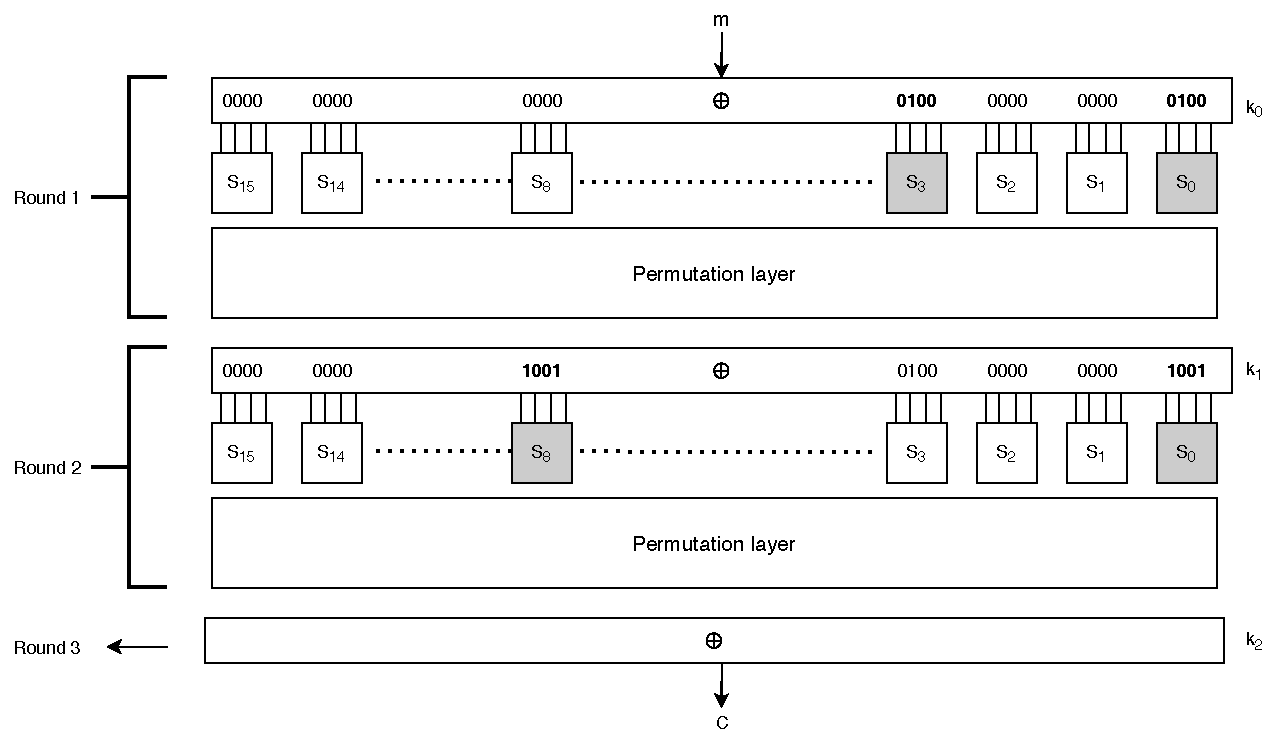
\includegraphics[width=\linewidth]{DC1.pdf}
        \endminipage
        \caption{Attack Model}
    \end{figure}
\end{frame}

\begin{frame}{The Difference Distribution Table}
\begin{figure}[h!]
    \caption{DDT of the S-box}
    \centering
    \scalebox{0.8}{
    \begin{tabular}{ |c||c|c|c|c|c|c|c|c|c|c|c|c|c|c|c|c| }
        \hline
         & 0 & 1 & 2 & 3&4& 5& 6&7&8&9&A&B&C&D&E&F  \\ \hline \hline
         0& 16 & 0 & 0 & 0 &0 &0 &0 &0& 0& 0 &0& 0& 0 &0& 0& 0 \\ 
         1& 0 & 0 & 0 & 4 & 0 & 0 & 0 & 4 & 0 & 4 &0& 0& 0 &4& 0& 0 \\
         2& 0 & 0 & 0 & 2 & 0 & 4 & 2 & 0 & 0 & 0 &2& 0& 2 &2& 2& 0 \\
         3& 0 & 2 & 0 & 2 & 2 & 0 & 4 & 2 & 0 & 0 &2& 2& 0 &0& 0& 0 \\
         4& 0 & 0 & 0 & 0 & 0 & 4 & 2 & 2 & 0 & 2 &2& 0& 2 &0& 2& 0 \\
         5& 0 & 2 & 0 & 0 & 2 & 0 & 0 & 0 & 0 & 2 &2& 2& 4 &2& 0& 0 \\
         6& 0 & 0 & 2 & 0 & 0 & 0 & 2 & 0 & 2 & 0 &0& 4& 2 &0& 0& 4 \\
         7& 0 & 4 & 2 & 0 & 0 & 0 & 2 & 0 & 2 & 0 & 0 & 0 & 2 & 0 & 0 & 4\\
         8& 0 & 0 & 0 & 2 & 0 & 0 & 0 & 2 & 0 & 2 & 0 & 4 & 0 & 2 & 0 & 4\\
         9& 0 & 0 & 2 & 0 & 4 & 0 & 2 & 0 & 2 & 0 & 0 & 0 & 2 & 0 & 4 & 0\\
         A& 0 & 0 & 2 & 2 & 0 & 4 & 0 & 0 & 2 & 0 & 2 & 0 & 0 & 2 & 2 & 0\\
         B& 0 & 2 & 0 & 0 & 2 & 0 & 0 & 0 & 4 & 2 & 2 & 2 & 0 & 2 & 0 & 0\\
         C& 0 & 0 & 2 & 0 & 0 & 4 & 0 & 2 & 2 & 2 & 2 & 0 & 0 & 0 & 2 & 0\\
         D& 0 & 2 & 4 & 2 & 2 & 0 & 0 & 2 & 0 & 0 & 2 & 2 & 0 & 0 & 0 & 0\\
         E& 0 & 0 & 2 & 2 & 0 & 0 & 2 & 2 & 2 & 2 & 0 & 0 & 2 & 2 & 0 & 0\\
         F& 0 & 4 & 0 & 0 & 4 & 0 & 0 & 0 & 0 & 0 & 0 & 0 & 0 & 0 & 4 & 4\\ \hline
    \end{tabular}
    }
\end{figure}
\end{frame}

\begin{frame}{Differential Characteristics}
\begin{table}[h!]
	\caption{Characteristics}
	\centering
	\begin{tabular}{ |c||c|c|c| }
		\hline
		Rounds & & Diff. & Prob. \\ \hline \hline
		I& & $x_0 = 4$, $x_4 = 4$ &  \\ 
		$R_1$& $k_0$ & $x_0 = 4$, $x_4 = 4$ & 1 \\
		$R_1$& S & $x_0 = 5$, $x_{3} = 5$ & $2^{-4}$ \\
		$R_1$& P & $x_0 = 9$, $x_{8} = 9$ & 1 \\
		$R_2$& $k_1$ & $x_0 = 9$, $x_{8} = 9$ & 1 \\ \hline
	\end{tabular}\\
\end{table}
\begin{block}{Characteristic}
        ($x_0 = 4$, $x_3 = 4$) $\xrightarrow[]{\text{R}}$ ($x_0 = 9$, $x_8 = 9$)
    \end{block}
\end{frame}


\begin{frame}{Idea of filtering}
\begin{itemize}
        \item Decrease Wrong pair $\xrightarrow[]{}$ Idea of filtering
        \item Observe from the DDT that transitions from $9 \xrightarrow[]{} \{2,4,6,8,c,e\}$
        \item Thus, after the effect of permutation layer of the second round, $c_1 \oplus c_2$ must belong to the set given below : \\ 
        $\{\{x_4=1,x_6=1\},\{x_6=1,x_8=1\},\{x_4=1,x_6=1,x_8=1\},\{x_6=1,x_{12}=1\},\{x_6=1,x_8=1,x_{12}=1\},...\}$ We have written code for this.
    \end{itemize}
    \begin{block}{Filtering}
        Thus, message pair leading to the cipher text difference other than the above set, can be discarded. 
        So, after filtering only $2^{14}$ plaintext pairs are left in our case.
    \end{block}
\end{frame}

\begin{frame}{Key Guess}
\begin{figure}[H]
	\centering
	\minipage{\textwidth}
	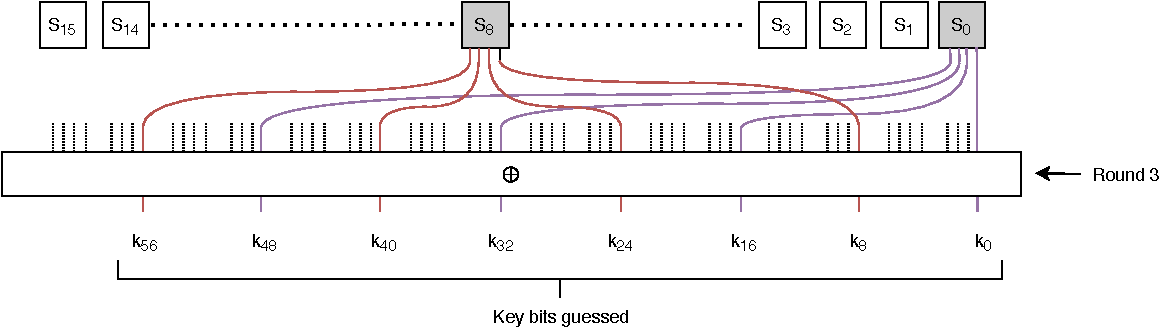
\includegraphics[width=\linewidth]{DC2.pdf}
	\endminipage
	\caption{Guess 8 bits of the key $k_2$}
	\label{fig:dc2}
\end{figure}\\
We are able to find 8 bits of key $k_2$. In our case only  8 bit right  subkey holds for all $2^{14}$ filtered pairs or in other word highest counter indicate the right 8 bit subkey.
\end{frame}

\begin{frame}{Complexity Analysis}
    \begin{block}{Complexity}
    \textbf{(Data, Time, Memory)} = $(2^{19},2^{25.17},2^{14})$
    \end{block}
\end{frame}
